\documentclass{scrartcl}

\usepackage[utf8]{inputenc}

\usepackage{fixltx2e}

% Step environment
% <https://tex.stackexchange.com/a/12943/13262>
\usepackage{amsthm}
\newtheorem*{remark}{Remark}
%
\newtheoremstyle{named}{}{}{\itshape}{}{\bfseries}{.}{.5em}{\thmnote{#1 }#3}
\theoremstyle{named}
\newtheorem*{step}{Step}

\usepackage{microtype}
\usepackage{amsmath}
\usepackage{mathtools}
\usepackage{booktabs}
\usepackage{tabularx}

\usepackage{pgfplots}
\pgfplotsset{compat=newest}

\usepackage{siunitx}

\newcommand\mytitle{Remarks on the conversion from OSA-UCS to CIEXYZ}
\newcommand\myauthor{Nico Schlömer}

\usepackage[
  pdfencoding=unicode,
  ]{hyperref}
\hypersetup{
  pdfauthor={\myauthor},
  pdftitle={\mytitle}
}

% <https://tex.stackexchange.com/a/43009/13262>
\DeclarePairedDelimiter\abs{\lvert}{\rvert}%

\usepackage[T1]{fontenc}
\usepackage{newtxtext}
\usepackage{newtxmath}

% degree symbol
\usepackage{gensymb}

% % <https://tex.stackexchange.com/a/413899/13262>
% \usepackage{etoolbox}
% \makeatletter
% \long\def\etb@listitem#1#2{%
%   \expandafter\ifblank\expandafter{\@gobble#2}
%     {}
%     {\expandafter\etb@listitem@i
%      \expandafter{\@secondoftwo#2}{#1}}}
% \long\def\etb@listitem@i#1#2{#2{#1}}
% \makeatother

% Okay. Don't use biblatex/biber for now. There are breaking changes in every
% revision, and we'd have to stick to the exact version that arxiv.org has,
% otherwise it's error messages like
% ```
% Package biblatex Warning: File 'main.bbl' is wrong format version
% - expected 2.8.
% ```
% \usepackage[sorting=none]{biblatex}
% \bibliography{bib}

\usepackage{amsmath}
\DeclareMathOperator{\sign}{sign}

\usepackage{bm}
\newcommand\rgb{\bm{R}}

\title{\mytitle\footnote{The LaTeX sources of this article are on \url{https://github.com/nschloe/colorio}}}
\author{\myauthor}

\begin{document}

\maketitle
\begin{abstract}
  This
\end{abstract}

In 1974, MacAdam published the definition of the OSA-UCS colorspace~\cite{macadam} that
tries to adhere particularly well to experimentally measured color distances, and
represents work that had been going on since the late 1940s.  One aspect of OSA-UCS is
the fact that the conversion from CIEXYZ coordinates into OSA-UCS Lgj coordinates is
straightforward, but the conversion the other way around is not. In fact, there is no
conversion method that works purely in elementary functions. Apparently, this had not
been a design goal of OSA-UCS.

In 2002, Kobayasi and Yosiki presented an OSA-UCS-to-CIEXYZ algorithm that leverages
Newton's method for solving nonlinear equation systems~\cite{kobayasi}. While the
algorithm is mostly in order, the article remains vague at important points and also
contains false assertions about the nature of the involved functions.

In 2013, Cao et al.\ compared Kobayasi's approach with some other, more complicated
methods based on artificial neural networks and found the latter to be
superior~\cite{cao}.

In the present note, the author aims to iron out the inaccuracies in Kobayasi's article
and shows that the Newton-based approach is indeed fully sufficient for the conversion
from OSA-UCS to CIEXYZ.

\section{The forward conversion}

The conversion from CIEXYZ coordinates to OSA-UCS Lgj coordinates is definied as
follows:

\begin{itemize}
  \item Compute $x$, $y$ coordinates via
    \[
      x = \frac{X}{X + Y + Z},\quad y = \frac{Y}{X + Y + Z}.
    \]
  \item Compute $K$ and $Y_0$ as
    \[
      \begin{split}
        K &= 4.4934 x^2 + 4.3034 y^2 - 4.276 x y - 1.3744 x - 2.5643 y + 1.8103,\\
        Y_0 &= Y K
      \end{split}
    \]

  \item Compute $L'$ and $C$ as
    \begin{equation}\label{eq:lc}
      \begin{split}
        L' &= 5.9 \left(\sqrt[3]{Y_0} - \frac{2}{3} + 0.042 \sqrt[3]{Y_0 - 30}\right)\\
        C &= \frac{L'}{5.9 \left(\sqrt[3]{Y_0} - \frac{2}{3}\right)}.
      \end{split}
    \end{equation}
    Note that $L'$ is $L$ in the original article~\cite{macadam}.

  \item Compute RGB as
    \[
      \begin{bmatrix}
        R\\
        G\\
        B
      \end{bmatrix}
      =
      M
      \begin{bmatrix}
        X\\
        Y\\
        Z
      \end{bmatrix}
    \]
    with
    \[
      M=\begin{bmatrix}
        +0.7990 & 0.4194 & -0.1648\\
        -0.4493 & 1.3265 & +0.0927\\
        -0.1149 & 0.3394 & +0.7170
      \end{bmatrix}.
    \]

  \item Compute $a$, $b$ as
    \[
      \begin{bmatrix}
        a\\
        b
      \end{bmatrix}
      =
      A
      \begin{bmatrix}
        \sqrt[3]{R}\\
        \sqrt[3]{G}\\
        \sqrt[3]{B}
      \end{bmatrix}
    \]
    with
    \[
      A = \begin{bmatrix}
        -13.7 & +17.7 & -4\\
        1.7 & +8 & -9.7
      \end{bmatrix}.
    \]

  \item Compute Lgj as
    \[
      \begin{split}
        L &= \frac{L' - 14.3993}{\sqrt{2}},\\
        g &= Ca,\\
        j &= Cb.
      \end{split}
    \]
\end{itemize}

\section{The backward conversion}

This section describes the conversion from the  $L$, $g$, $j$ to the $X$, $Y$, $Z$
coordinates and mostly sticks to Kobayasi~\cite{kobayasi} here.

Given $L$, we can first compute
\[
  L' = L \sqrt{2} + 14.3993.
\]
Equation~\ref{eq:lc} gives the nonlinear relationship between $L'$ and $Y_0$ from which
we will retrieve $Y_0$. First set $t\coloneqq \sqrt[3]{Y_0}$ and solve $f(t)=0$ for $t$
using Newton's method with
\[
  \begin{split}
    f(t) &\coloneqq {\left(\frac{L'}{5.9} + \frac{2}{3} - t\right)}^3 - 0.042^3 (t^3 - 30)\\
    f'(t) &= -3 {\left(\frac{L'}{5.9} + \frac{2}{3} - t\right)}^2 - 0.042^3 3 t^2.
  \end{split}
\]
It is reasonable to assume that
\[
  t_0 = \frac{L'}{5.9} + \frac{2}{3}
\]
is a good initial guess for $t$ since the second term in $f(t)$ with $0.042^3$ is
probably small.
Indeed, in practical application it takes less than 10 Newton iterations to achieve
convergence up to a tolerance of $10^{-13}$.

From here, one can compute
\[
  Y_0 = t^3,\quad
  C = \frac{L'}{5.9 \left(t - \frac{2}{3}\right)},\quad
  a = \frac{g}{C},\quad
  b = \frac{j}{C}.
\]


\begin{figure}
  \centering
  \hfill
  % This file was created by tikzplotlib v0.8.5.
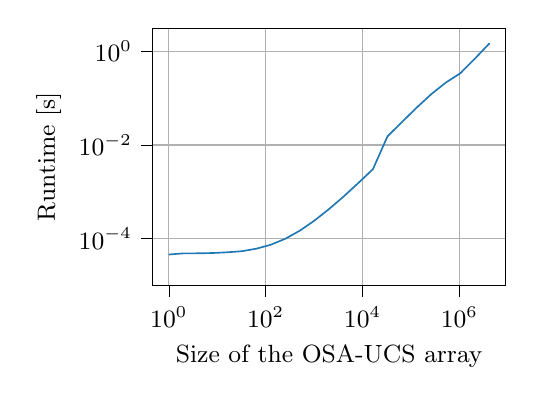
\begin{tikzpicture}
\small
\definecolor{color0}{rgb}{0.12156862745098,0.466666666666667,0.705882352941177}

\begin{axis}[
width=0.5\textwidth,
height=0.4\textwidth,
log basis x={10},
log basis y={10},
tick align=outside,
tick pos=left,
x grid style={white!69.01960784313725!black},
xmajorgrids,
xmin=0.466516495768404, xmax=8990687.44201965,
xmode=log,
xtick style={color=black},
y grid style={white!69.01960784313725!black},
xlabel={Size of the OSA-UCS array},
ylabel={Runtime [s]},
ymajorgrids,
ymin=1.0e-05, ymax=3.0946896171257,
ymode=log,
ytick style={color=black}
]
\addplot [semithick, color0]
table {%
1 4.6026e-05
2 4.8656e-05
4 4.8798e-05
8 4.9518e-05
16 5.1298e-05
32 5.406e-05
64 6.1218e-05
128 7.4422e-05
256 0.000100108
512 0.00014922
1024 0.000244824
2048 0.000432382
4096 0.000798368
8192 0.00154504
16384 0.003041107
32768 0.015252678
65536 0.03102277
131072 0.062590365
262144 0.121108512
524288 0.214264196
1048576 0.339891653
2097152 0.697448122
4194304 1.476815604
};
\end{axis}

\end{tikzpicture}

  \hfill
  % This file was created by tikzplotlib v0.8.5.
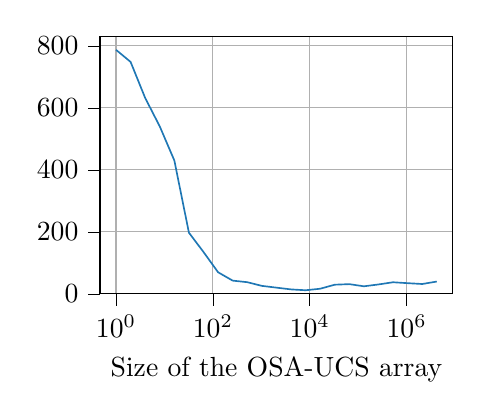
\begin{tikzpicture}

\definecolor{color0}{rgb}{0.12156862745098,0.466666666666667,0.705882352941177}
\definecolor{color1}{rgb}{1,0.498039215686275,0.0549019607843137}

\begin{axis}[
width=0.5\textwidth,
height=0.4\textwidth,
log basis x={10},
tick align=outside,
tick pos=left,
x grid style={white!69.01960784313725!black},
xmajorgrids,
xmin=0.466516495768404, xmax=8990687.44201965,
xmode=log,
xtick style={color=black},
y grid style={white!69.01960784313725!black},
% ylabel={Runtime relative to cbrt},
ymajorgrids,
ymin=0, ymax=830,
ytick style={color=black},
xlabel={Size of the OSA-UCS array}
]
\addplot [semithick, color0]
table {%
1 787.066433566434
2 748.043062200957
4 631.69647696477
8 540.053088803089
16 430.216724738676
32 197.28831378892
64 135.024555079973
128 69.6830099941211
256 42.7417648170309
512 37.6977113374785
1024 25.8176709590747
2048 20.1362440723177
4096 14.446842284113
8192 11.6819040387925
16384 16.5864959757117
32768 29.5641483554035
65536 31.3942138250337
131072 24.4242208227254
262144 30.4130064747132
524288 37.476925997706
1048576 34.5039382592277
2097152 31.8295473370856
4194304 39.7625721082598
};
\end{axis}

\end{tikzpicture}

  \hfill
  \caption{This is a caption.}
\end{figure}

% \printbibliography{}
\bibliography{main}{}
\bibliographystyle{plain}

\end{document}
